\documentclass[border=2mm]{standalone}
\usepackage{tikz}
\usetikzlibrary{calc,patterns,angles,quotes}
\begin{document}
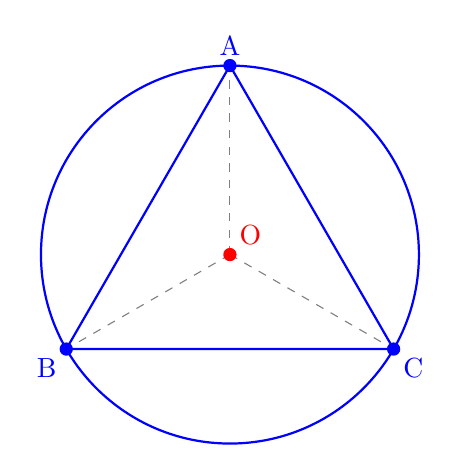
\begin{tikzpicture}[scale=0.8]
    \coordinate (O) at (0,0);
    \draw[blue, thick] (O) circle (3);
    \draw[blue, thick] (90:3) coordinate (A) -- (210:3) coordinate (B) -- (330:3) coordinate (C) -- cycle;
    \draw[dashed,gray] (O)--(A);
    \draw[dashed,gray] (O)--(B);
    \draw[dashed,gray] (O)--(C);
    \fill[blue] (A) circle (3pt) node[above] {A};
    \fill[blue] (B) circle (3pt) node[below left] {B};
    \fill[blue] (C) circle (3pt) node[below right] {C};
    \fill[red] (O) circle (3pt) node[above right] {O};
\end{tikzpicture}
\end{document}